\subsection{UC12 - Rimozione plug-in}
\begin{figure}[H]
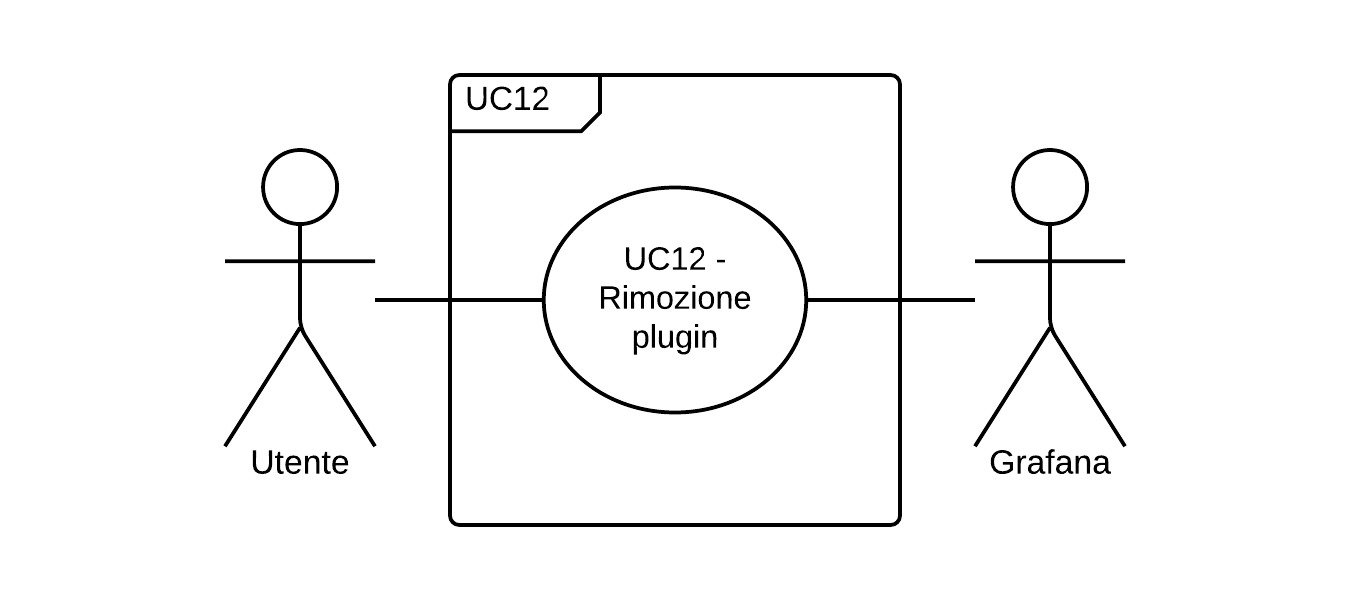
\includegraphics{img/UC12_-_Rimozione_plugin.png}
\caption{Diagramma degli use case di UC12}
\end{figure}
\begin{itemize}
    \item \textbf{Codice identificativo}: UC12;
    \item \textbf{Titolo}: rimozione plug-in;
    \item \textbf{Attori primari}: utente;
    \item \textbf{Attori secondari}: Grafana\glo;
    \item \textbf{Descrizione}: l'utente rimuove il pannello di Grafana\glosp dove è inserito il plug-in provocandone l'arresto e successivamente la rimozione;
    \item \textbf{Precondizioni}: l'utente è autenticato nel sistema software Grafana\glosp e ha avviato il plug-in;
    \item \textbf{Postcondizioni}: l'utente ha rimosso con successo il plug-in da Grafana\glo;
    \item \textbf{Scenario principale}: l'utente rimuove il pannello di Grafana\glosp in cui è inserito il plug-in provocandone la rimozione.
\end{itemize}